
\section{Analysis and Comparisons over Prior methods}

In the algorithm, we make a heap of data units that will reduce seek time by
just moving instead of copying them. We perform these moves first before
working with data units that need copying. This initial step will produce a
better solution than proposed by \cite{cacheobliviouslayout} without adding
redundant units. This result is possible mainly because our optimization
algorithm searches wider sets of potential locations for moving cases in an
efficient manner.
%mowhere data
%units are close to each other but in hierarchically different blocks in
%\cite{cacheobliviouslayout}. 
To show this, consider a case where we have two
access requirements of 5 data units each. Figure \ref{YoonImprovement} shows an
example of that kind of layout. In the middle of that figure is the result of
using the cache oblivious layout. Because it hierarchically constructs blocks
and arranges the units in each block, it does
not detect that the
units with the black access requirement can be grouped together. On the other
hand, the algorithm we propose would shorten the black access requirements
without adding redundancy, as shown in the bottom of that figure.

\begin{figure}[ht]
\centering
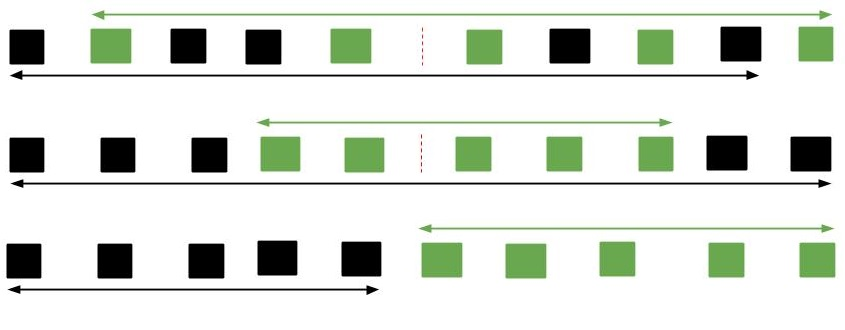
\includegraphics[width=\columnwidth]{ImprovementOverYoon.jpg}
\caption{Example of two access requirements of 5 data units each. The red line represents the boundary between blocks in the cache oblivious layout hierarchy. The original layout (top), cache-oblvious layout (middle), as well as the layout after running our algorithm (bottom) is shown.}
\label{YoonImprovement}
\end{figure}

The algorithm in \cite{cacheobliviouslayout} did not necessarily produce the best cache oblivious mesh layout. However, even if we had the best layout without redundancy, we would actually achieve a better seek time than it using redundancy. We have such an example with Figure \ref{fig:startingProb}. As can be seen in the figure, the total seek time is 7 units which turns out to be the minimum possible seek time without redundancy, as found through a brute-force search. With redundancy, the total seek time is the minimum required which is 6 units. While a reduction from 7 to 6 units may not seem dramatic, when this result is scaled up to the hundreds of millions, this makes a big difference in seek time, which we saw in practice.\\

\begin{figure}[h!]
\centering
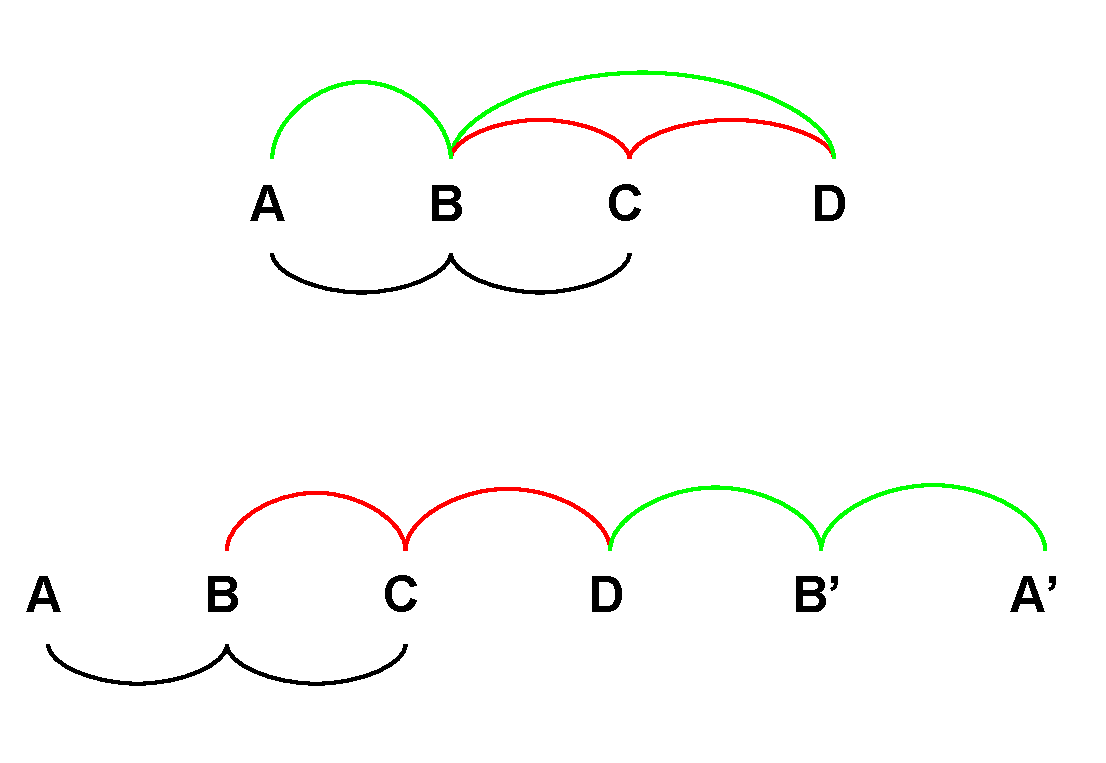
\includegraphics[width=\columnwidth]{DataLayoutPaper_TheoryLayouts.pdf}
\caption{Data Units with varying access requirements on the top. The letters represent data units and each color represents a different access requirement. It is laid out in its optimal layout without redundancy on top. A layout with redundancy and minimal EST is shown at the bottom}
\label{fig:startingProb}
\end{figure}

